\section{Durchführung}
\label{sec:Durchführung}
Der experimentelle Aufbau ist in Abbildung \ref{fig:Aufbau} zu sehen, wobei zusätzlich noch ein PC angeschlossen ist, mit 
dem der Versuchsaufbau angesteuert wird. Die relevanten Komponenten bestehen aus einer Kupfer Röntgenröhre, die bei einer Spannung von 35kV
und einem Emissionsstrom von 1mA betrieben wird. Die nächste wichtige Komponente ist der LiF-Kristall mit einem 
Gitterabstand $d=\qty{201.4}{\pico\meter}$ an der die Röntgenstrahlung gemäß der Bragg-Bedingung gebeugt wird.
Für die Detektion wird ein Geiger-Müller Zählrohr auf dem Goniometer installiert.
\begin{figure}[H]
    \centering
    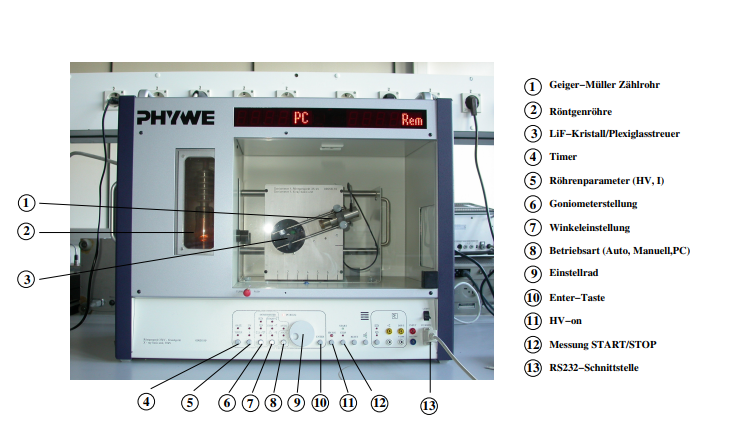
\includegraphics[scale=1]{content/Aufbau.png}
    \caption{Versuchsaufbau\cite{sample}.}
    \label{fig:Aufbau}
\end{figure}

\noindent Im ersten Versuchsteil ging es darum mit dem gegebenen Versuchsaufbau die 
Braggbedingung zu verifizieren. Dafür wird der Kristall in einem festen Kristallwinkel von $\theta=14°$
fest eingestellt. Da die Braggbedingung nun ein Maximum bei dem doppelte Winkel $\alpha=28°$
vorhersagt, wird der Geigermüllerzähler im Winkelbereich zwischen 26° bis 30° in 0,1° Schritten 
variiert. Dabei wird pro Winkel für $\qty{5}{\s}$ detektiert. Es werden wie bei allen Messungen in diesem
Praktikumsversuch die Anzahl der Detektionen in Abhängigkeit des Messwinkels gemessen.
\\
\noindent Nun soll das Emissionsspektrum der Cu-Röntgenröhre untersucht werden.
Dafür soll jetzt die Wellenlängenabhängigkeit der gemessenen Intensität gemessen werden. Dafür werden
jetzt Kristall und Messwinkel im Verhältnis 1:2 gekoppelt. 
Zunächst wird das Spektrum grob aufgenommen. Dafür wird im Kristallwinkelbereich von 4° bis 26°
bei einer Integrationszeit von $\qty{5}{\s}$ in 0,2° Schritten die Intensität gemessen.
Mit der Kenntnis aus der groben Messung kann nun im Winkelbereich  das Detailspektrum 
$K_\alpha$ und $K_\beta$ genauer aufgelöst werden. Es wird dabei wieder in 0.1° Schritte 
und bei einer Integrationszeit von $\qty{5}{\s}$ gemessen.
\\
\noindent Als letztes soll die Messapparatur dafür verwendet werden, um die Absorptionsenergie der K-Kante und
die Abschirmzahl von vier verschiedenen Anodenmaterialien zu bestimmen. Dabei soll in 0.1° Schritte mit $\qty{20}{\s}$ 
Integrationszeit gemessen werden. Die Absorber werden auf den Geiger-Müller geschraubt. Es sind Zink mit $Z=30$, Brom $Z=35$,
Strontium mit $Z=38$ und Gallium mit $Z=31$ gemessen worden. Die Winkelbereiche sind so gewählt worden, dass 1° vor angefangen und 1° nach dem 
theoretischen Kanten Winkel aufgehört wird. Der kritische Winkel von Zink ist bei 18,6°, der für Brom bei 13,2°, von Strontium bei 16,12° und 
der von Gallium bei 17,22°.




